\documentclass[11pt]{article}
    
\usepackage{amsmath}
\usepackage{amsfonts}
\usepackage{cite}
\usepackage[letterpaper, total={6.5in, 9in}]{geometry}
\usepackage{mathpazo}
\usepackage{sourcecodepro}
\usepackage{graphicx}
\usepackage{hyperref}

\newcommand{\setcomp}[2]{\left\{ #1 \ \Big|\ #2 \right\}}
\newcommand{\rngto}[1]{1{:}#1}
\newcommand{\abs}[1]{\left| #1 \right|}
\newcommand{\absdet}[1]{\abs{#1}}
\newcommand{\dv}[1]{\mathrm{d}{#1}}
\newcommand{\Exp}{\mathrm{Exp}}
\newcommand{\vect}{\mathrm{vec}}
\newcommand{\vectu}{\mathrm{vecu}}

\begin{document}


\title{Efficient Unconstraining
  Parameter Transforms for Hamiltonian Monte Carlo}
\author{Meenal Jhajharia \\ \small Flatiron Institute 
\and Seth Axen \\ \small University of T\"ubingen 
\and Adam Haber \\ \small Weizmann Institute 
\and Sean Pinkney \\ \small Omnicom Media Group
\and Bob Carpenter \\ \small Flatiron Institute}
\date{DRAFT: \today}
\maketitle


\begin{abstract}
  \noindent
  This paper evaluates the statistical and computational
  efficiency of unconstraining parameter transforms for Hamiltonian
  Monte Carlo sampling.
\end{abstract}

\section{Introduction}

In statistical computing, we often need to compute high-dimensional
integrals over densities $\pi(x)$ (e.g., Bayesian estimation or
prediction, $p$-value calculations, etc.).  The only black-box
techniques that work for general high-dimensional integrals are
Markov chain Monte Carlo (MCMC) methods.  The most effective MCMC
method in high dimensions is Hamiltonian Monte Carlo (HMC).  HMC works
by simulating the Hamiltonian dynamics of a fictitious particle
representing the value being sampled coupled with a momentum term.

Although it is possible to write HMC samplers that work for simply
constrained values such as upper- and/or lower-bounds
\cite{neal2011mcmc} or unit vectors \cite{byrne2013geodesic}, it is
much more challenging to do the same for complex constraints such as
simplexes or positive definite matrices or for densities involving
multiple constrained values.  Instead, it is far more common to map
the constrained values to unconstrained values before sampling
\cite{JSSv076i01}.  For example, the Probabilistic  Programming language Stan, defines distributions with an unconstrained support, in favour of making sampling an easier process. The variables with constraints (or with constrained support in this case) are transformed to an unconstrained space. Inverse transforms of these variables are used for log density adjustments. These are usually in the form of a Jacobian matrix comprised of the gradient $\frac{\partial x}{\partial y}$, where $x$ and $y$ are the constrained and unconstrained parameters respectively.

These gradients are computationally expensive, certain transforms are entirely inefficient, and some work well on certain distributions or parametrizations and vice versa. This presents the issue of selecting which transform to use
among an infinite set of options, which is the topic of this paper. We begin by defining the general theory of transforms, followed by transforms from a unit simplex $\Delta^N$ to the $R^M$. Finally, we discuss notions of "better" transforms defined on the simplex, using statistical measures like Effective Sample Size, Leapfrog steps taken by the sampler etc.




\section{Unconstraining Transforms}

To draw samples from a parameter defined on a constrained space $\mathcal{X}$ that can be uniquely parameterized by $n$ real degrees of freedom, we instead perform sampling in an unconstrained space $\mathcal{Y} \in \mathbb{R}^m$ for $m \ge n$. Let $p_Y(y)$ be an improper density function defined over $\mathcal{Y} \rightarrow(0, \infty)$ with support over all elements of $\mathcal{Y}$ and a surjective, smooth and continuous map $g: \mathcal{Y} \rightarrow \mathcal{X}$. Then, for any proper density $\pi_{X}$ over $\mathcal{X}$, the constraining transform can be defined as $\left(p_{Y}, g\right)$: $\mathcal{Y} \rightarrow \mathcal{X}$. In this case, the density $p_{Y}(y)=\pi_{Y}(y) \cdot \pi_{X}(g(y))$ is proper, and $Y \sim \pi_Y \implies g(Y) \sim \pi_X$. The required change of variables for this unconstraining transform is:
\[
  p_Y(y) = p_X(f^{-1}(y)) \absdet{J_{f^{-1}}(y)},
\]
where the Jacobian of the inverse transform is defined by
\[
  J_{f^{-1}}(y) = \frac{\partial}{\partial y} \, f^{-1}(y)
\]


In this paper we consider transforms where $m = n$, for which the constraining transform is defined as $(\pi_Y, f)$: $\mathcal{Y} \rightarrow \mathcal{X}$, given that $\pi_{Y}(y)=\absdet{J_{f^{-1}}(y)}$.



\section{Unit simplex}


%A simplex is a set of non negative vectors that sum up to a constant $a$, this can be written as:
%\begin{equation*}
%\Delta=\left\{\mathbf{x} \in \mathbb{R}^{n} \mid\left\langle\mathbf{x}, \mathbf{1}_{n}\right\rangle=a, \mathbf{x} \geq 0\right\}
%\end{equation*}
%
%In computational works, we generally care about the unit simplex, this is the special case where $ a = 1$. Geometrically, an \textit{n-simplex} is the convex closure of $n+1$ affinely independent set of points $x_0, x_1, \dots x_n$. It is the simplest polytope for $n$-dimensions (in this case we will be looking at a simplex as a convex polytope, not abstract). An \textit{n-simplex} is be represented in the barycentric coordinate system with weighted vertices, as follows:
%\begin{equation*}
%\Delta = \left\{x_{0} u_{0}+\cdots+x_{n} u_{n} \mid \sum_{i=0}^{n} x_{i}=1\\
% \text{ and } x_{i} \geq 0 \text { for } i=0, \ldots, k\right\}
%\end{equation*}
%
%With this representation, taking $u_{i}=1$, the $n$ unit simplex can be written as: 
%\begin{equation*}
%\left\{x \in \mathbb{R}^{n}: x_{0}+\cdots+x_{n-1}=1, x_{i} \geq 0 \text { for } i=0, \ldots, k-1\right\}
%\end{equation*}
%
%A \textit{unit simplex} on $R^n$ is an $n - 1$ dimensional simplex with unit vectors as vertices. Notice the unit weights, this set only has $n-1$ affinely independent points.
%
%Sum to one constraints are useful in probabilistic inference, often used for modeling categorical responses. The rest of the section describes various transforms used to map a simplex to an unconstrained space ($R^n$).\\
%\\

A unit $N$-simplex is an $N + 1$-dimensional vector of non-negative
values that sums to one.  Simplexes are useful for representations of multinomial probabilities
(e.g., probabilities of categories in a classification problem). The set of unit $N$-simplexes is conventionally denoted
\[
  \Delta^N = \setcomp{x \in \mathbb{R}_{\ge 0}^{N + 1}}{ \sum_{i=1}^{N} x_i = 1}
\]
Geometrically, an $N$-simplex is the convex closure of $N+1$ points
that are 1 in one coordinate and 0 elsewhere.  For example, the
3-simplex is the complex closure of
$\begin{bmatrix}1 & 0 & 0 \end{bmatrix},
\begin{bmatrix} 0 & 1 & 0 \end{bmatrix}$,
and $\begin{bmatrix} 0 & 0 & 1 \end{bmatrix}$. As such, there are only $N$ degrees of
freedom, because if $x$ is an $N$-simplex, then
\[
  x_N = 1 - (x_1 + x_2 + \cdots + x_{N-1}).
\]
We will use $\Delta^N_-$ to denote $N-1$ elements of a simplex, this is sufficient to uniquely determine $\Delta^N$.
\subsection{StickBreaking Transform}

The StickBreaking transform carries forward the intuition in the stick-breaking construction for Dirichlet \cite{sethuraman1994constructive}. It is a process of recursively breaking a piece $x_i$ from a stick of unit length, where the leftover stick in the $i^{th}$ iteration is $ 1 - \sum_{1}^{i}x$. Let $y = f(x)$, then we define the stick-breaking mapping $ f \colon \Delta^{N-1} \xrightarrow{\makebox[0.4cm]{$\sim$}}  R^{N-1}$, for $1 \leq i \leq N$ as:	
\[
y_i
= \mathrm{logit}(z_i) - \mbox{log}\left(\frac{1}{N-i}
   \right) 
   \]
  
for break proportion 
\[ 
 z_i = \frac{x_i}{1 - \sum_{i' = 1}^{i-1} x_{i'}}.
\]\\

The inverse transform $ f^{-1} \colon R^{N-1} \xrightarrow{\makebox[0.4cm]{$\sim$}}  \Delta^{N-1}$ is defined as:

\[
x_i = \left( 1 - \sum_{i'=1}^{i-1} x_{i'} \right)\\
\]

for break proportion \[z_i = \mathrm{logit}^{-1} \left( y_i  + \log \left( \frac{1}{N - i}
                                            \right)\right)
                                            \]\\
                                            
                                            
An $N$ dimensional unit simplex $\Delta^{N-1}$ has $N-1$ degrees of freedom (Notice that this inverse transform only maps the first $N-1$ elements, the last element of the simplex $x_{N} = 1 - \sum_1^{N-1}{x_i}$). The Jacobian matrix for $f^{-1}$ is a lower-triangular diagonal matrix, so for the change of variables we evaluate $\mathbf{J}_{i, i}$ where $i \in 1:N-1$.
\begin{align*}
\mathbf{J}_{i, i} &= \frac{\partial x_i}{\partial y_i}
=
\frac{\partial x_i}{\partial z_i} \,
\frac{\partial z_i}{\partial y_i}\\
\mathbf{J}_{i, i} &= \left(
  1 - \sum_{k' = 1}^{k-1} x_{k'}
   \right) z_k (1 - z_k),\\
   \abs{\, det \, \textbf{J} \,} &= \prod_{i=1}^{N-1} \textbf{J}_{i,i}
\end{align*}

The correction term $p_Y(y) = p_X(f^{-1}(y))\,
\prod_{i=1}^{N-1}z_i\,(1 - z_i)\left(1 - \sum_{i'=1}^{i-1} x_{i'}\right).$
\subsection{Additive log ratio transform}

The unconstraining transform for the identified softmax is known as
the additive log ratio (ALR) transform
\cite{aitchison1982statistical}, which is a bijection
$\textrm{alr}:\Delta^{N-1} \rightarrow \mathbb{R}^{N-1}$ defined for
$x \in \Delta^{N-1}$ by
\[
  \textrm{alr}(x)
  = \begin{bmatrix}\displaystyle
    \log \frac{x_1}{x_N} \cdots \log \frac{x_{N-1}}{x_N}
  \end{bmatrix}
\]
The inverse additive log ratio transform maps values in
$\mathbb{R}^{N-1}$ to $\Delta^{N-1}$ defined for $y \in
\mathbb{R}^{N-1}$ by
\[
  \textrm{alr}^{-1}(y)
  = \textrm{softmax}(\begin{bmatrix} y &  0 \end{bmatrix}),
\]
where for $u \in \mathbb{R}^N$,
\[
  \textrm{softmax}(u) = \frac{e^u}{\sum{e^u}}
\]
Again, the change of variables adjustment is calculated for $N-1$ dimensions.  
\[
\begin{bmatrix}
    \textrm{alr}^{-1}(y)_1
    & \cdots &
    \textrm{alr}^{-1}(y)_{N-1}
    \end{bmatrix} = \frac{e^y}{\sum e^y + 1}
\]
From a density $p_X(x)$ defined over $x \in \Delta^{N-1}$,
we can obtain a density over unconstrained parameters $y \in
\mathbb{R}^{N-1}$ by applying the inverse ALR transform and adjusting
for the change of variables
\[
  p_Y(y) = p_X(\textrm{alr}^{-1}(y)) \absdet{J_{f^{-1}}(y)}
\]
where $J_{f^{-1}}$ is the $N-1$ dimensional Jacobian matrix. To calculate the determinant of the Jacobian of the inverse transform,
we start by noting that $alr^{-1}(y) = f \circ g$, where
$f(y) = e^{ \circ y}$ (elementwise exponential), and $g(z)=\frac{z}{\sum z + 1}$. Here $z = e^{\circ y} \in R_{+}^{N-1}$, at this point we evaluate the Jacobian as:
\[
  \absdet{J_{alr^{-1}}(y)}
  = \absdet{J_{f(y)}} \absdet{J_{g(z)}}
\]
Note that $J_{f(z)}$ only consists of diagonal entries $e^{y_{i}}$
\[
  \absdet{J_{f(y)}} = \prod_i^n e^{y_i}
\]
For $g$ we begin with evaluating $ J_{g} = \frac{\partial g(z)}{\partial z}$. Note that $\mathbf{1}$ is a vector of ones.
\[
 J_g = \frac{1}{1 + \sum e_{i=1}^{N} z_i} \mathbb{I}_{N-1}
  - \left(\frac{1}{1 + \sum e_{i=1}^{N} z_i^2} x \right)
  \mathbf{1}_{N-1}
\]
Using the matrix determinant lemma,\footnote{The matrix determinant lemma
  is \[\textrm{det}(A + u v^{\top}) = (1 + v^{\top} A^{-1} u)
    \textrm{det}(A).\]}
\begin{eqnarray*}
  |J_{g}|
  & = &
  \left(
    1
    + \mathbf{1}
    \left(\frac{1}{1 + \sum e_{i=1}^{N} z_i} \mathbb{I} \right)^{-1}
    \frac{-z}{(1 + \sum e_{i=1}^{N} z_i)^2}
    \right)
    \abs{\frac{1}{1 + \sum e_{i=1}^{N} z_i} \mathbb{I}}
  \\[6pt]
  
  & = & \left( \frac{1}{1 + \sum e_{i=1}^{N} z_i} \right)^N.
\end{eqnarray*} 
Finally,
\[
  \absdet{J_{alr^{-1}}(y)}
  \ = \
 \prod_i^n e^{y_i}
  \, \left( \frac{1}{1 + \sum e_{i=1}^{N}y_i} \right)^N.
\]
Putting $J_{alr^{-1}}$ in the change of variables adjustment, we get
\[
  p_Y(y)
  = p_X(\textrm{alr}^{-1}(y))
  \, \prod_{i=1}^{N} e^y_i)
  \left( \frac{1}{1 + \sum_{i=1}^{N} e^y_i}\right)^N
\]  

%\subsection{Softmax Transform}
%
%The softmax function can be understood from Multinomial Logistic
%Regression employed for predicting probabilities of a Categorically
%distributed variable. Geometrically it maps $R^K$ to the boundary of a
%unit K-simplex(it is simply the convex hull of $k+1$ affinely
%independent points in $R^K$. Essentially it transforms a vector of
%size K to another vector of size K where the outputs sum to 1. It is
%worth noting that the mapping is actually from $R^K$ to $R^{K-1}$, so
%when a vector of size $K$ is transformed the $K_th$ vector is simply
%$1$- sumof k-1 vectors


\subsection{Simplex softmax parameterization}

We define the transformation
$\phi: \mathbb{R}^{n-1} \to \Delta^n_-: y \mapsto x_-$, where
$x=\begin{pmatrix}x_- \\ \frac{1}{r}\end{pmatrix} \in \Delta^n$,
$x_i = \frac{1}{r} e^{y_i}$ for $1 \le i \le n-1$, and
$r = 1 + \sum_{i=1}^{n-1} e^{y_i}$.

First we compute the scalar derivatives:
\[
\begin{aligned}
  \frac{\mathrm{d} r}{\mathrm{d} y_j}
  &= e^{y_j} = r x_j\\
  \frac{\mathrm{d} x_i}{\mathrm{d} y_j}
  &= \delta_{ij} \frac{1}{r} e^{y_i} - \frac{1}{r^2} e^{y_i}
  \frac{\mathrm{d} r}{\mathrm{d} y_j}
  = \delta_{ij} x_i - x_i x_j, \quad 1 \le i \le n-1
\end{aligned}
\]
where
$\delta_{ij} = \begin{cases} 1 &\text{if } i = j \\ 0
  &\text{otherwise}\end{cases}$ is the Kronecker delta.

If $\mathrm{diag}(x)$ is the diagonal matrix whose diagonal are the
elements of $x$, then the Jacobian is
\[
  J = (I_{n-1} - x_- \boldsymbol{1}_{n-1}^\top) \operatorname{diag}(x_-),
\]
where $\boldsymbol{1}_n$ is the $n$-vector of ones.

Using Sylvester's determinant theorem,
$|I_{n-1} - x_- \boldsymbol{1}_{n-1}^\top| = 1 -
\boldsymbol{1}_{n-1}^\top x_- = 1 - \sum_{i=1}^{n-1} x_i = x_n$, so
$$\mathrm{correction} = |J| = x_n \prod_{i=1}^{n-1} x_i = \prod_{i=1}^{n} x_i = \exp\left(\sum_{i=1}^{n-1} y_i\right) \left(1 + \sum_{i=1}^{n-1} e^{y_i}\right)^{-n}$$


\subsection{Simplex softmax parameterization through parameter expansion}

We define the transformation
$\phi: \mathbb{R}^n \to \Delta^{n-1} \times \mathbb{R}_{>0}: y \mapsto
(x_-, r)$, where $r = \sum_{i=1}^n e^{y_i}$ and
$x_i = \frac{1}{r} e^{y_i}$ for $1 \le i \le n-1$..

First we compute the scalar derivatives:
\[
\begin{aligned}
  \frac{\mathrm{d} r}{\mathrm{d} y_j}
  &= e^{y_j} = r x_j
  \\
  \frac{\mathrm{d} x_i}{\mathrm{d} y_j}
  &= \delta_{ij} \frac{1}{r} e^{y_i} - \frac{1}{r^2} e^{y_i} \frac{\mathrm{d} r}{\mathrm{d} y_j} = \delta_{ij} x_i - x_i x_j,
\end{aligned}
\]
which corresponds to the Jacobian
\[
  J = \begin{pmatrix}I_{n-1} - x_- \boldsymbol{1}_{n-1}^\top & -x_- \\
    r \boldsymbol{1}_{n-1}^\top & r \end{pmatrix} \mathrm{diag}(x).
\]

For invertible $A$, the determinant of the block matrix
$\begin{pmatrix}A & B \\ C & D\end{pmatrix}$ is $|A| |D-CA^{-1}B|$.  A
square matrix is invertible iff its determinant is non-yero.  From the
previous section,
\[
  |I_{n-1} - x_- \boldsymbol{1}_{n-1}^\top| = x_n > 0,
\]
so the determinant of the Jacobian is
\[
  |J| = x_n \left|r + r \boldsymbol{1}_{n-1}^\top (I_{n-1} - x_-
    \boldsymbol{1}_{n-1}^\top)^{-1} x_-\right|
  \prod_{i=1}^n x_i.
\]

Let $w = (I_{n-1} - x_- \boldsymbol{1}_{n-1}^\top)^{-1} x_-$. Then,
\[
\begin{aligned}
    w - x_- \sum_{i=1}^{n-1} w_i &= x_-\\
    w &= x_- \left(1 - \sum_{i=1}^{n-1} w_i\right)\\
    \sum_{i=1}^{n-1} w_i &= \sum_{i=1}^{n-1} \left( x_- (1 - \sum_{i=1}^{n-1} w_i) \right) = \left(\sum_{i=1}^{n-1} x_i \right) \left(1 - \sum_{i=1}^{n-1} w_i\right) = (1 - x_n)  \left(1 - \sum_{i=1}^{n-1} w_i\right)\\
    \sum_{i=1}^{n-1} w_i &= \frac{1 - x_n}{x_n} = \frac{1}{x_n} - 1\\
    w &= x_- \left(1 - \left(\frac{1}{x_n} - 1\right)\right) = \frac{1}{x_n} x_-
  \end{aligned}
\]

Then
\[
  |J| = x_n r \left|1 + \frac{1}{x_n}\sum_{i=1}^{n-1} x_i\right|
  \prod_{i=1}^n x_i = r \prod_{i=1}^n x_i
\]

To keep the target distribution proper, we must select a prior
distribution $\pi(r)$ for $r$.  If we choose $r \sim \chi_n$, then the
product of the correction and the density of the prior for $r$ is
proportional to

\[
  \mathrm{correction}
  = \pi(r) |J| = r^n e^{-r^2/2} \prod_{i=1}^n x_i
  = \exp\left(\sum_{i=1}^n y_i - \frac{1}{2}\left(\sum_{i=1}^n
      e^{y_i}\right)^2\right).
\]

Alternatively, if we choose $r \sim \mathrm{Gamma}(n, 1)$, then
\[
  \mathrm{correction} = \pi(r) |J| = r^n e^{-r} \prod_{i=1}^n x_i =
  \exp\left(\sum_{i=1}^n y_i - \sum_{i=1}^n e^{y_i}\right).
\]
This latter correction is equivalent to the sampling procedure from
the Dirichlet distribution with $\alpha_i=1$, where
$z_i \sim \mathrm{Exponential}(1)$ and
$y = \frac{z}{\sum_{i=1}^n z_i}$.

Both of these corrections can be captured with the generalization
\[
  \mathrm{correction}
  = \pi(r) |J|
  = r^n e^{-r^p/p} \prod_{i=1}^n x_i
  = \exp\left(\sum_{i=1}^n y_i - \frac{1}{p} \left(\sum_{i=1}^n e^{y_i}\right)^p\right),
\]
for $p > 0$, which corresponds to $r \sim \text{Generalized-Gamma}(1, n, p)$.

\section{Results}

\begin{figure}
    \centering
    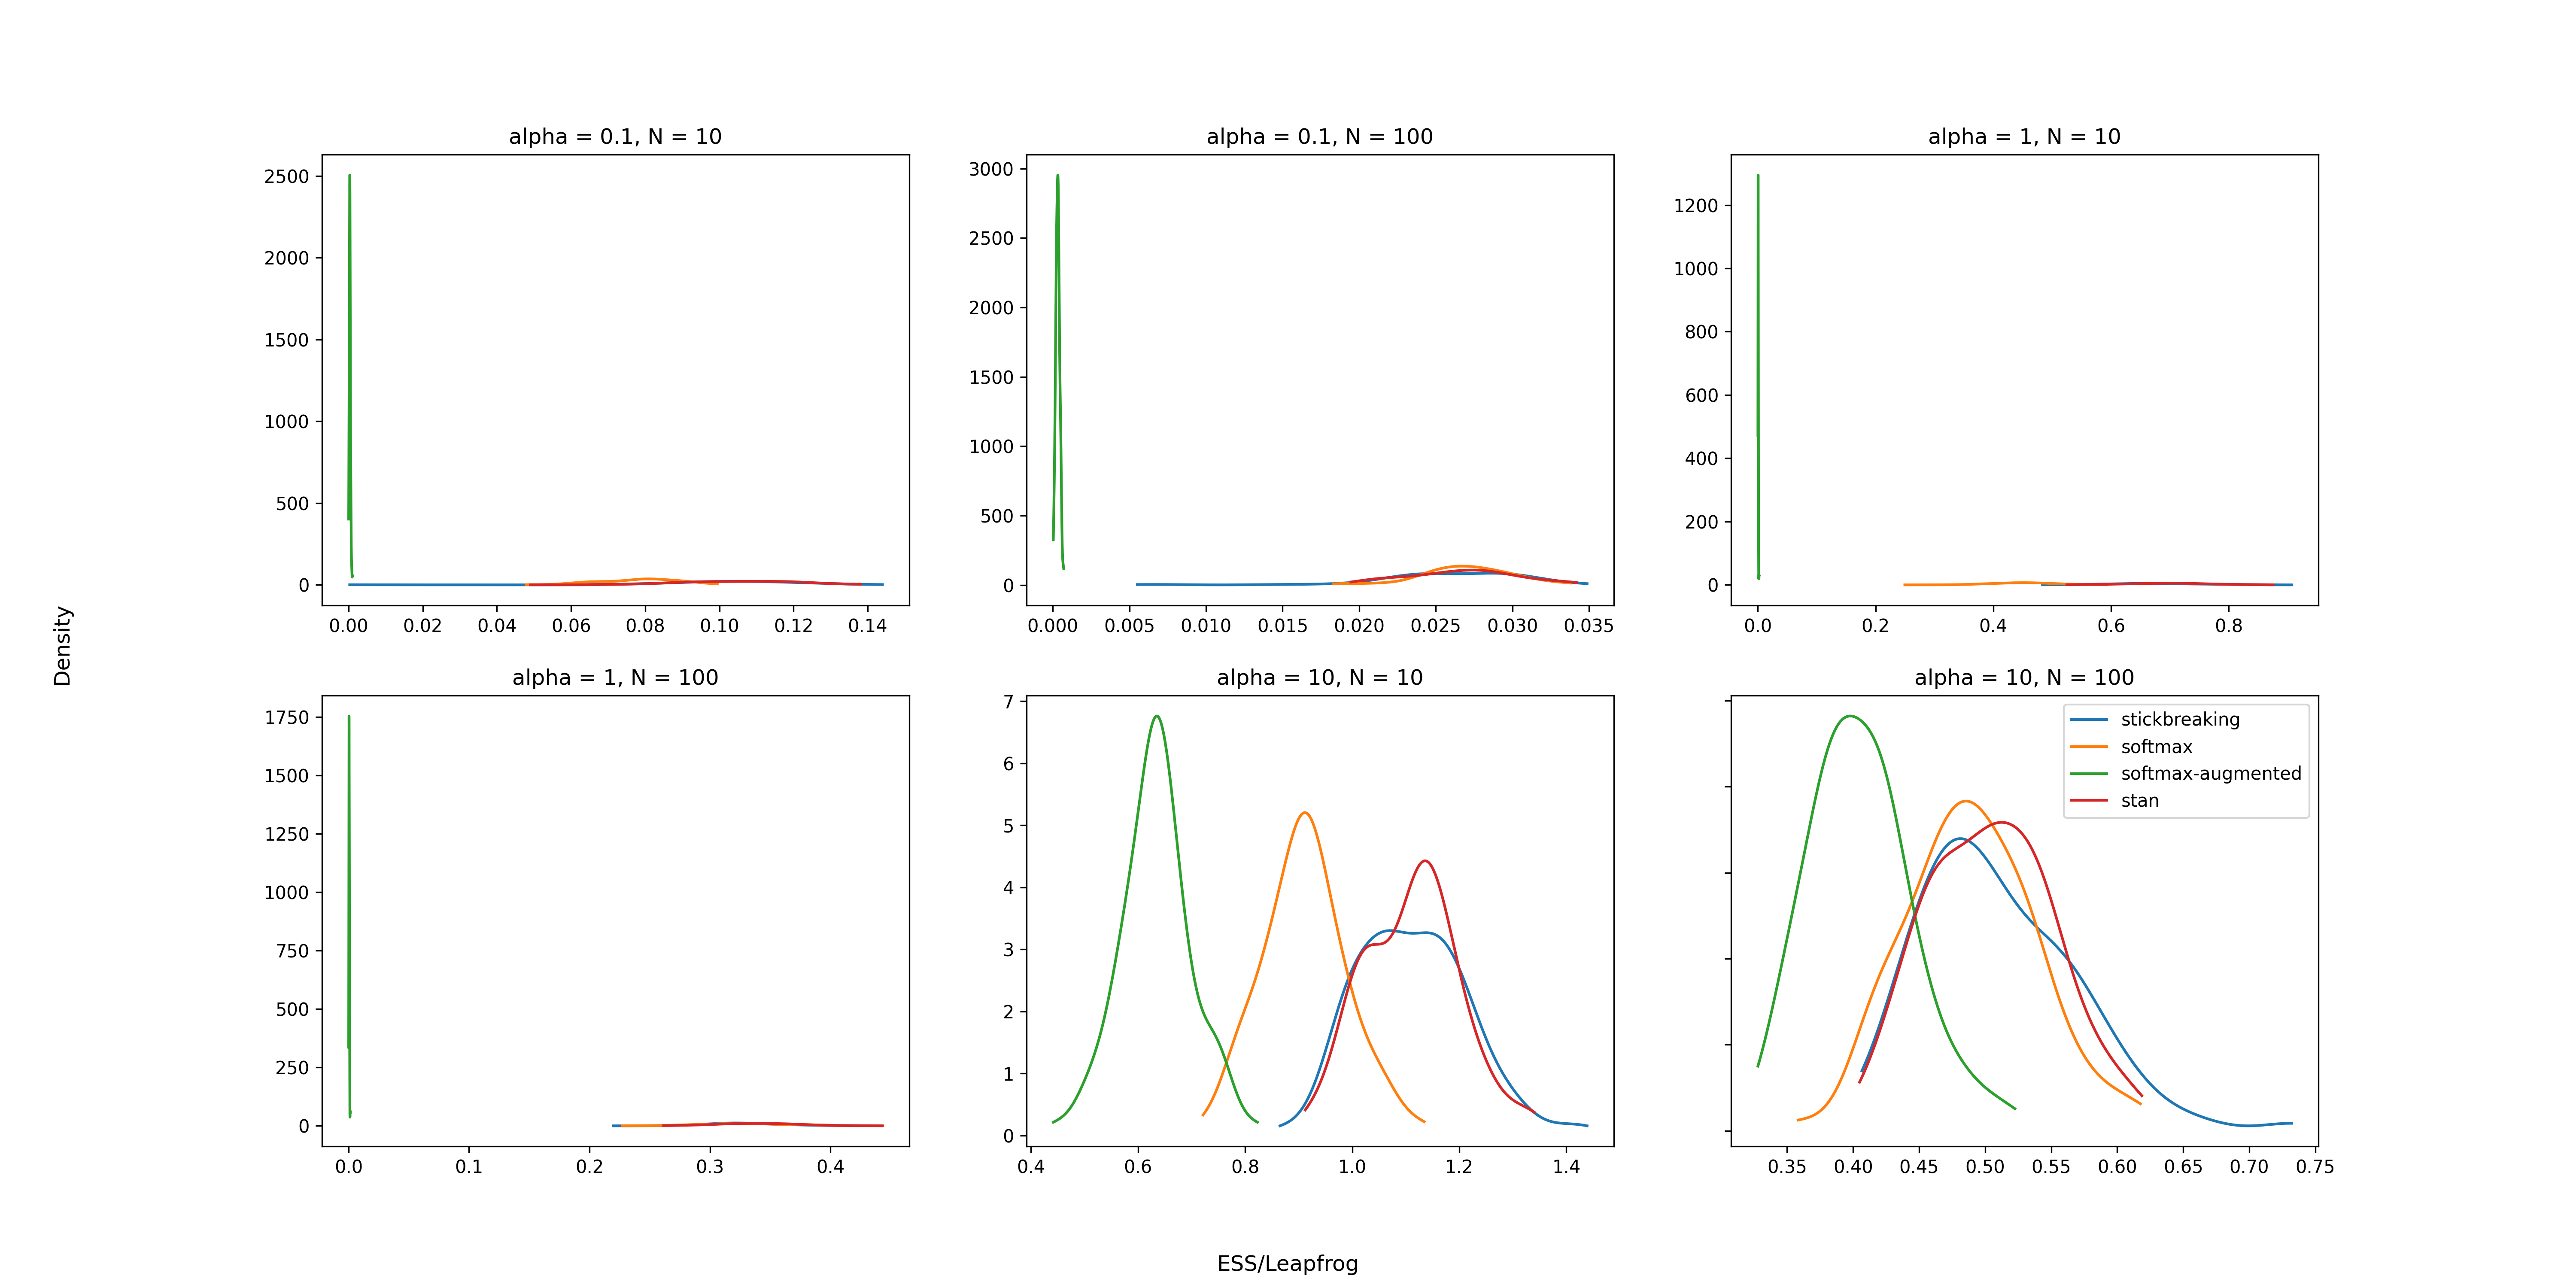
\includegraphics[width=1.2\textwidth]{figures/ess.png}
    \caption{Effective Sample Size vs Total LeapFrog Steps}
    \label{fig:ess}
\end{figure}

\begin{figure}
    \centering
    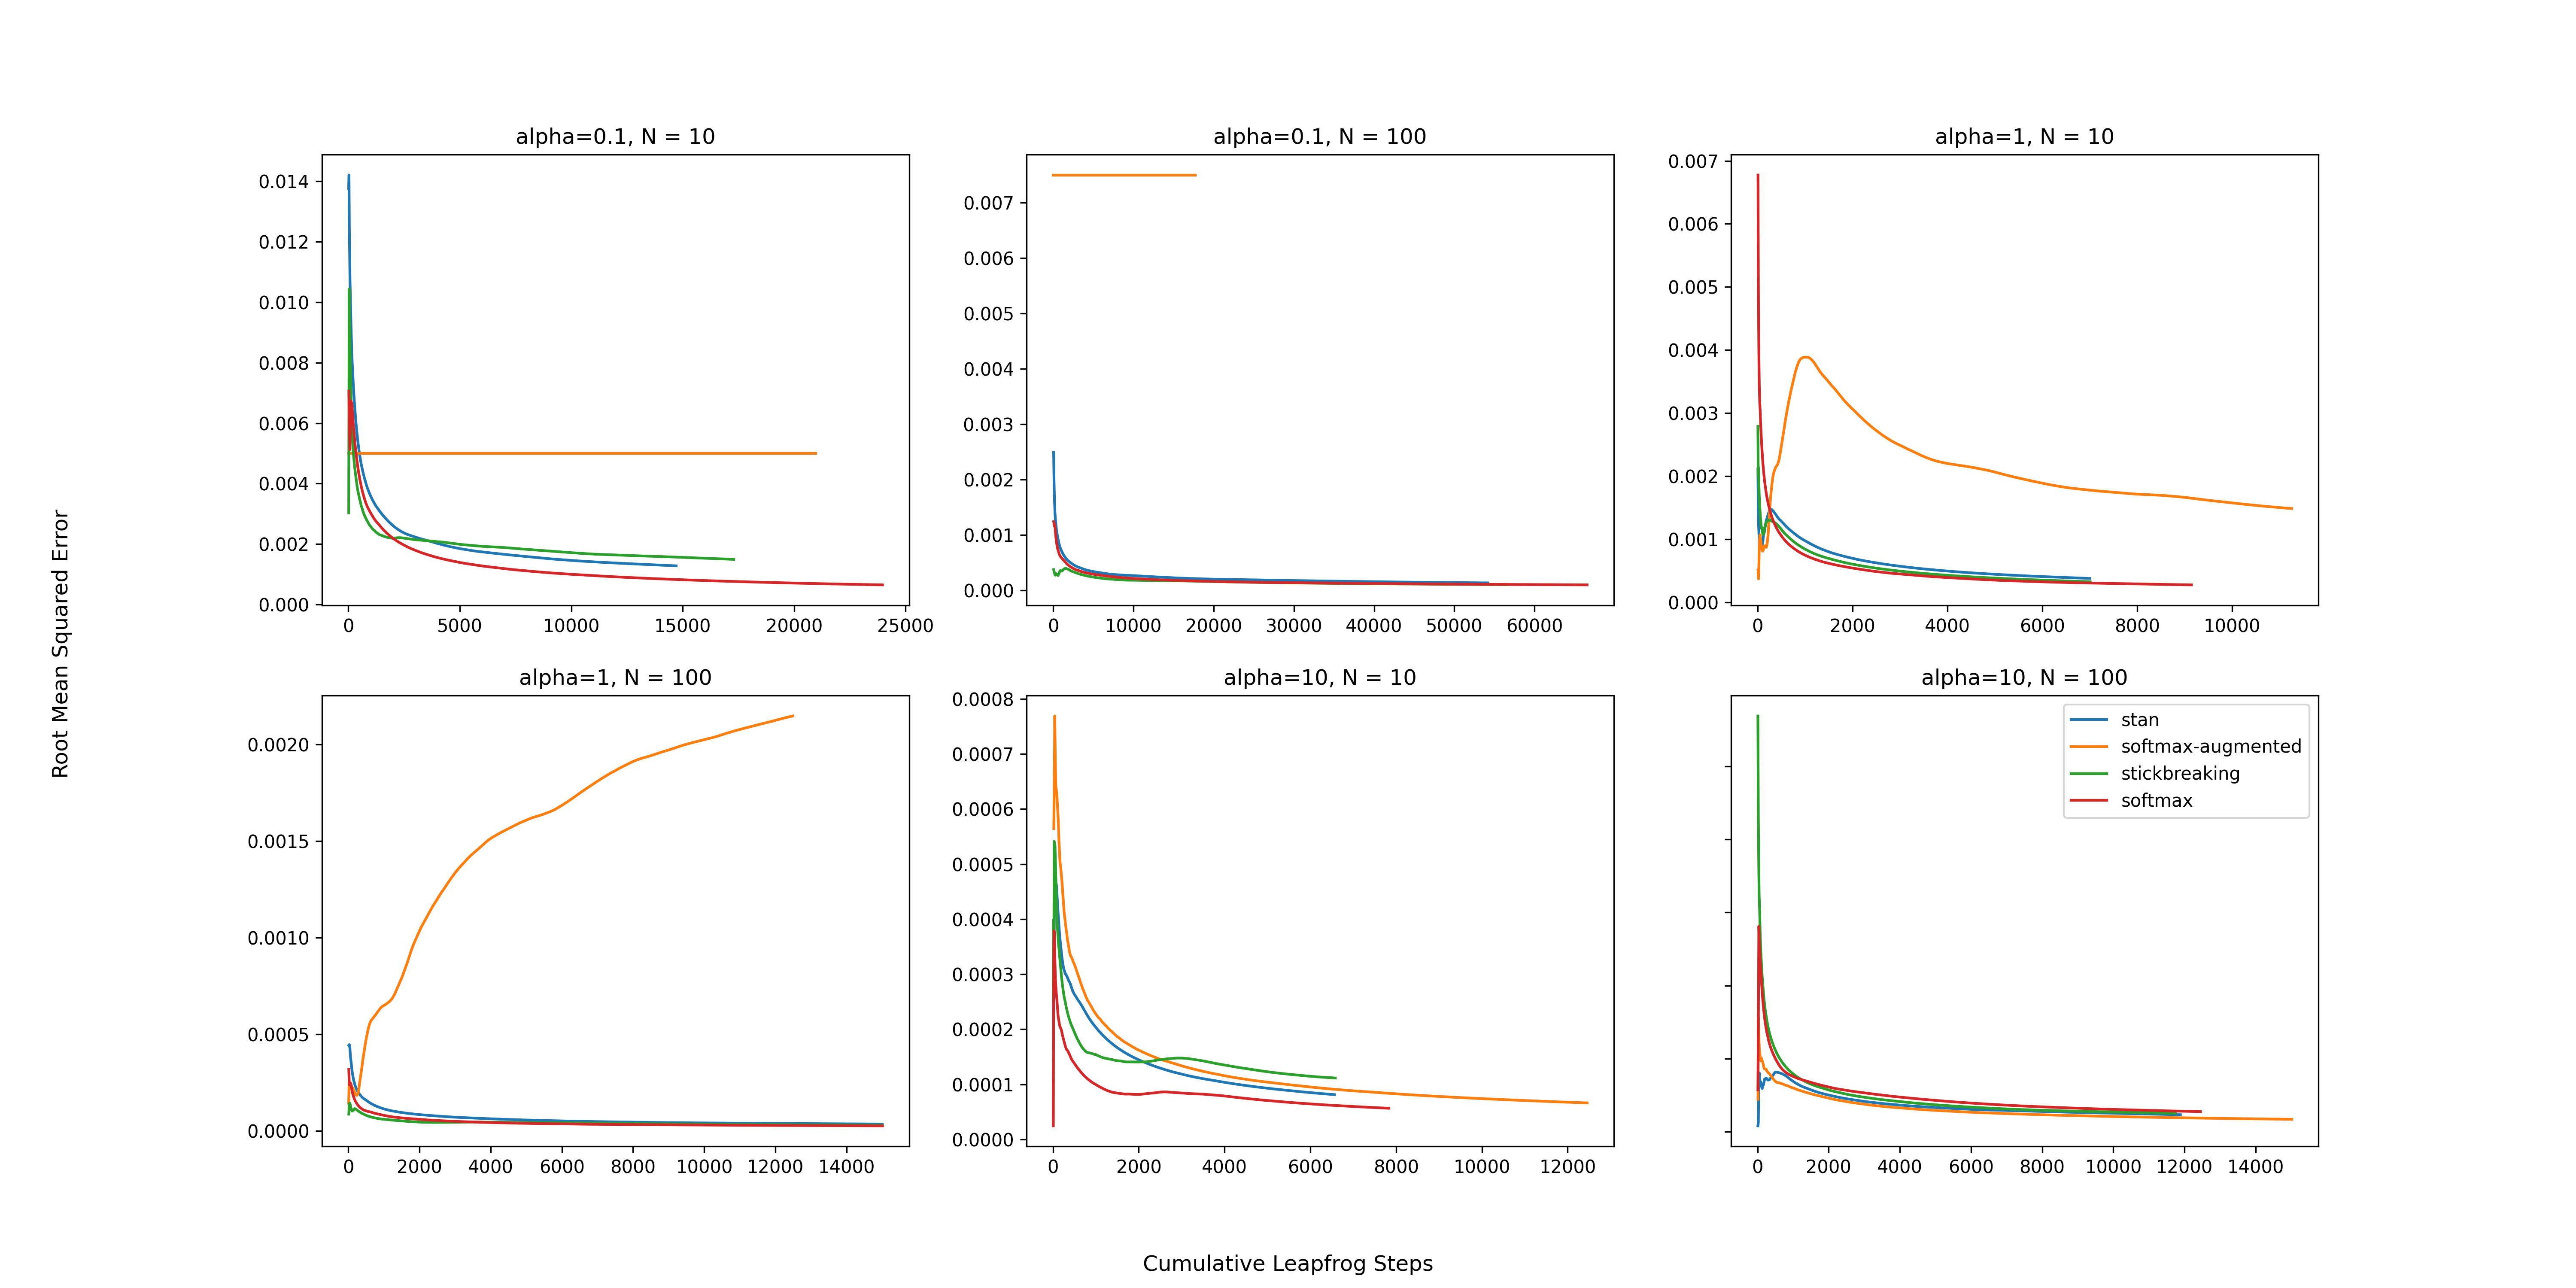
\includegraphics[width=1.2\textwidth]{figures/rmse.png}
    \caption{Root Mean Squared Error vs Cumulative Leapfrog Steps}
    \label{fig:rmse}
\end{figure}

\subsubsection*{Acknowledgements}

We would like to thank \url{matrixcalculus.org} for providing an
easy-to-use symbolic matrix derivative calculator.



\bibliography{all}{}
\bibliographystyle{plain}

\end{document}
